\documentclass[mathserif,t]{beamer}
%\usepackage{Sweave}                                                       
\usepackage{amssymb,bm,mathtools,amsmath}                                                      
\usepackage{graphicx,caption,float}
\usepackage[UKenglish]{isodate} % for: \today                             
\cleanlookdateon                % for: \today                             

\def\wl{\par \vspace{\baselineskip}\noindent}                             
\def\beginmyfig{\begin{figure}[ht]\begin{center}}                          
\def\endmyfig{\end{center}\end{figure}}                                   

\def\prodl#1#2#3{\prod\limits_{#1=#2}^{#3}}                               
\def\suml#1#2#3{\sum\limits_{#1=#2}^{#3}}                                 
\def\ds{\displaystyle}                                                    
\def\tbf#1{\textbf{#1}}
\def\inv{^{\raisebox{.2ex}{$\scriptscriptstyle-1$}}}
\def\pm{^{\raisebox{.2ex}{$\scriptscriptstyle\prime$}}}

% My Beamer Stuff
  \geometry{vmargin=0.3in} % Formating the top bar
  \newcommand{\m}[1]{\mathbf{\bm{#1}}} % Serif bold math
  %\beamertemplatenavigationsymbolsempty % To get rid of navigation bar

  % My Color Stuff
  \usepackage{xcolor} % http://en.wikibooks.org/wiki/LaTeX/Colors
                      % http://latexcolor.com/
    \definecolor{grey}{rgb}{0.15, 0.15, 0.15} % Sets default color. CHANGE THIS!
    \definecolor{pumpkin}{rgb}{1.0, 0.46, 0.09}
    \definecolor{darktan}{rgb}{1.0, 0.66, 0.07}
    \definecolor{coral}{rgb}{1.0, 0.5, 0.31}
    \pagecolor{grey} % Sets the bar color.

  \def\mylitecolor{coral}           % Bullet Color.       CHANGE THIS!
  \def\mycolor{\color{pumpkin}}     % Frame Title Color.  CHANGE THIS!
  \def\mydarkcolor{\color{darktan}} % Figure Color.       CHANGE THIS!
    \def\frametitle#1{\vspace{-.32in{\mycolor\textbf{#1}}}}
    \setbeamercolor{itemize item}{fg=\mylitecolor}
    \setbeamercolor{enumerate item}{fg=\mylitecolor}
    \setbeamercolor{itemize subitem}{fg=\mylitecolor}
    \setbeamercolor{itemize subsubitem}{fg=\mylitecolor}
    \setbeamercolor{title}{fg=\mylitecolor}
    %\setbeamercolor{figure}{fg=\mylitecolor}

    \usepackage[T1]{fontenc}
    \DeclareCaptionFont{figcol}{\mydarkcolor} 
    \captionsetup{
      labelfont={bf,figcol},
      %textfont={green}
    }

  %% my title:                                                               
  %\title[short title]{long title}
  %\logo{\includegraphics[width=1cm,height=1cm,keepspectration]{logo.pdf}
  %\author[Arthur Lui]{Arthur Lui}
  %\institute[Brigham Young University]{
  %  Department of Statistics\\
  %  Brigham Young University
  %}

%%%%%%%%%%%%%%%%



\begin{document}
% My Title: {
  \def\mytitle{\textbf{Predicting Germination Rates of Different Tulip
                       Populations at Various Chilling Times}}
  \title[Tulips]{\mytitle}
  \author[Arthur Lui]{Arthur Lui}
  \institute{
    Department of Statistics\\
    Brigham Young University
  }
  {
    %\setbeamercolor{background canvas}{bg=grey}
    \frame{\titlepage}
  }
%}

\frame{
  \frametitle{Tulips in the Netherlands}
  \beginmyfig
    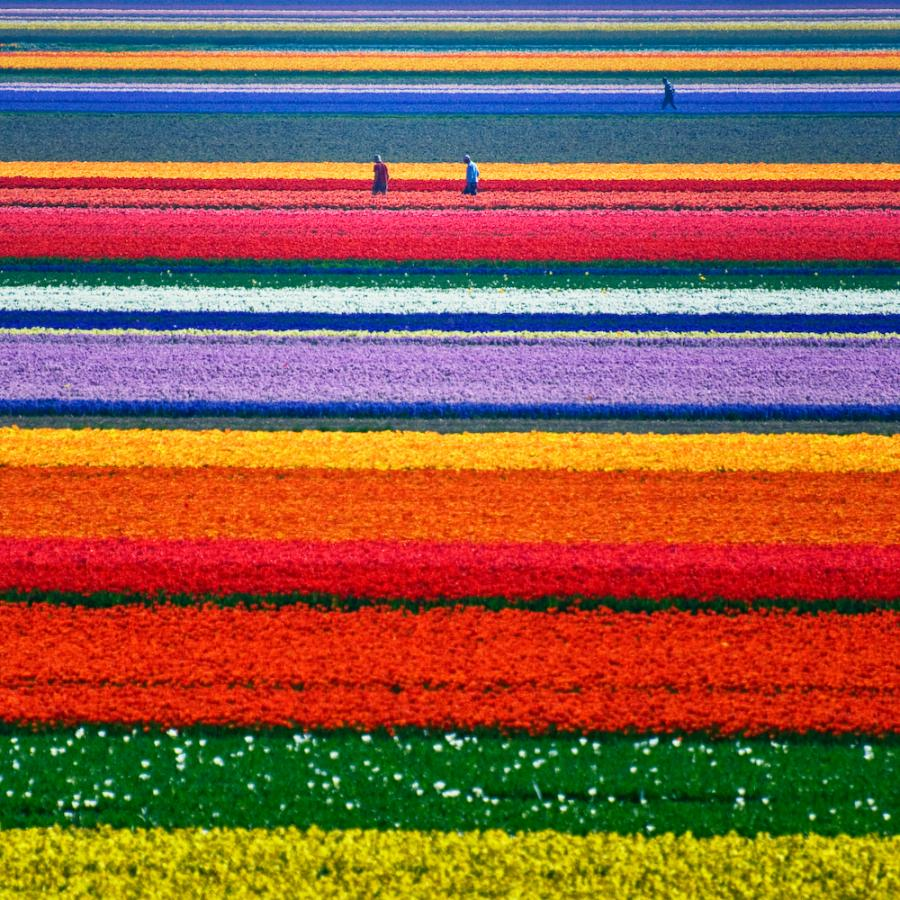
\includegraphics[scale=.21]{../../images/tulipsfieldsinholland6.jpg}
    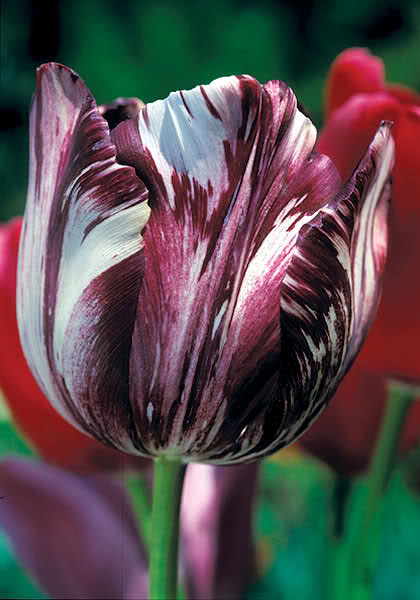
\includegraphics[scale=.21]{../../images/viceroy.jpg}
    \caption{Tulips popularized in the sixteenth century in Holland. During the 
             tulipomania, a viceroy (right) bulb could allegedly be exchanged for a basket
             of goods, some furniture, \textit{and} some live stock. Today, 9M bulbs
             are produced annually, and tulips account for 25\% of agricultural exports.}
  \endmyfig
}

\frame{
  \frametitle{How do we grow the most tulips?}
    \vspace{15mm}
    \begin{itemize}
      \item Most tulip seeds need 12-14 weeks of ``chill time'' (below 55$^\circ$F) before flowering \pause
      \item Various populations\footnote{\tiny https://github.com/luiarthur/Fall2014/tree/master/Stat637/project/tulip/data} 
            of tulip seeds react to chill times differently \pause
      \item[]
      \item Research Questions: \pause
      \begin{itemize}
        \item What is the effect of chilling time for each tulip population? \pause
        \item What is the optimal chill time for each tulip population? \pause
        \item How do the chill times differ by population?
      \end{itemize}
    \end{itemize}
}

\frame{
  \frametitle{Data}
  \beginmyfig
    \includegraphics[scale=.22]{../../images/allPopsData.pdf}
    \vspace{-2mm}
    \caption{Germination rates across all tulips for 7 chilling time (weeks). 
             Thirty measurements were made at each chilling time for each tulip population}
  \endmyfig
}

\frame{
  \frametitle{Data}
  \beginmyfig
    \includegraphics[scale=.22]{../../images/rawData.pdf}
    \vspace{-2mm}
    \caption{Germination rates of each tulip population by chilling times
             (weeks)}
  \endmyfig
}

\frame{
  \frametitle{Model}
  \vspace{15mm}
  \begin{tabular}{rl}
    $y_i  \sim$& \text{Bernoulli}($p_i$)\\
    $\Phi\inv(p_i) =$&$ \m{b(x_i)\beta}$ \\ \pause
                  $=$&$ \beta_0 + \suml{j}{1}{3}\beta_j b_j(x_i) \pause +
                        \suml{k}{1}{11} \beta_{0j}\cdot I\{\text{pop}_i=k\} \pause+ $\\
                $ $  &$ \suml{k}{1}{11} \suml{j}{1}{3}\beta_{1j}\cdot I\{\text{pop}_i=k\} b_j(x_i)$\\
                 &\\
                 \pause
    \text{Let $\m{W=b(X)}$,} & \\
    $\m{\beta}\sim$&$\text{Normal}\left(\m{W\pm\beta},\sigma_b^2\m{(W\pm W)\inv}\right)$
  \end{tabular}  
  \pause \wl\wl\wl
  Note that for this Bayesian probit model, we can make use of the Albert and Chib (1993) algorithm
  to obtain the posterior for $\m\beta$.
}

\frame{
  \frametitle{Results}
  \beginmyfig
    \includegraphics[scale=.22]{../../images/chilleffect.pdf}
    \vspace{-2mm}
    \caption{Predicted germination rates of each population of tulips by
             chilling times (weeks)}
  \endmyfig
}

{\setbeamercolor{background canvas}{bg=grey}
  \frame{
    \frametitle{The End}
    \vspace{30mm}
    \begin{center}
      \color{pumpkin}\Huge \textbf{Questions?}
    \end{center} 
  }
}

\end{document}
